%! Licence = CC BY-NC-SA 4.0

%! Author = gianfluetsch
%! Date = 22. Jan 2022
%! Project = icth_summary

\section{Digitale Modulationsarten}

\subsubsection{Prüfung HS2017}
Die Datensequenz $'1 1 1 0 0 0 0 1 0 1 0 1'$ wird bei einer festen Bitrate von 1 MBit/s mittels vier verschiedener Modulationsarten übertragen. Charakterisieren Sie die verwendeten Verfahren und stellen Sie jeweils die Wertigkeit M der Symbole, d.h. die Anzahl übertragener
Bits pro Symbol fest!
\begin{center}
    \vspace{-8pt}
    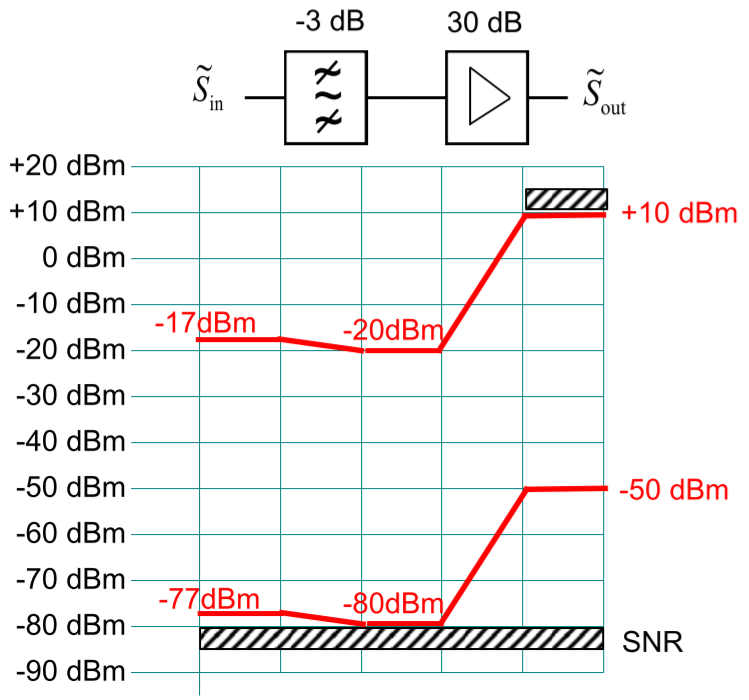
\includegraphics[width=.8\linewidth]{./12-modulationsarten/hs2017}
    \vspace{-8pt}
\end{center}
\begin{center}
    \vspace{-8pt}
    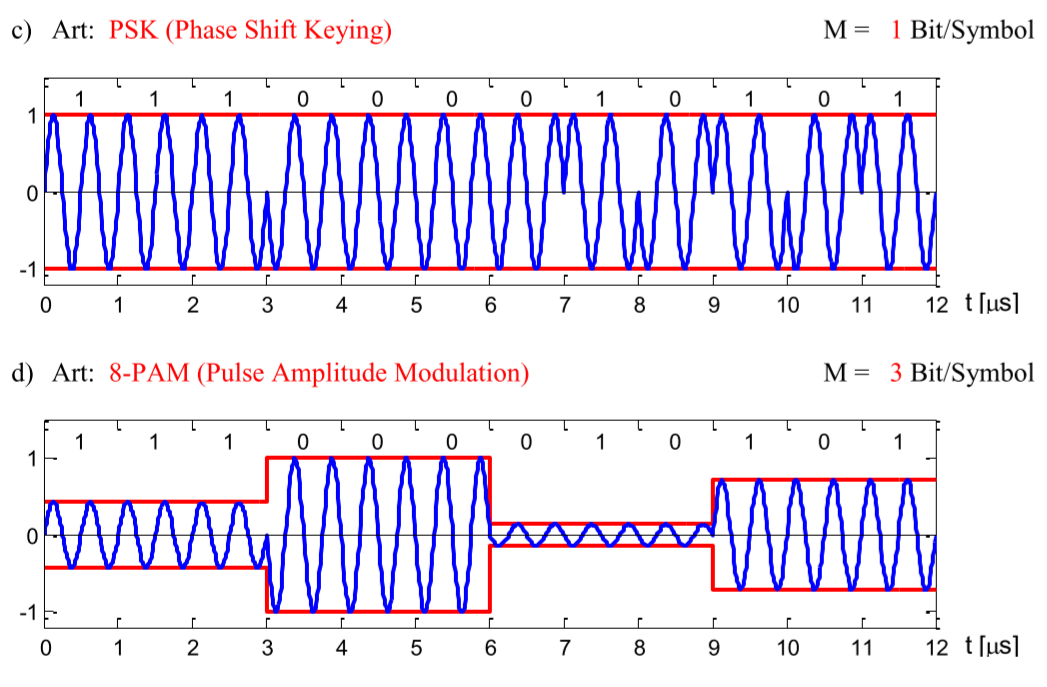
\includegraphics[width=.8\linewidth]{./12-modulationsarten/hs2017_1}
    \vspace{-8pt}
\end{center}